\documentclass[10pt,a4paper]{article}

% ---------- Codificación e idioma ----------
\usepackage[utf8]{inputenc}
\usepackage[T1]{fontenc}            % acentos y guiones bien en el PDF
\usepackage[english]{babel}
\DeclareUnicodeCharacter{2212}{-}   % el signo menos Unicode no rompe la compilación

% ---------- Página ----------
\usepackage[a4paper,margin=2cm]{geometry}   % 2 cm: límite de 2 páginas
\usepackage{microtype}              % mejor reparto de espacios, ahorra líneas

% ---------- Matemáticas ----------
\usepackage{amsmath,amssymb,amsthm}

% ---------- Unidades y química ----------
\usepackage{siunitx}
\sisetup{per-mode=symbol}           % kcal/mol en vez de kcal mol^-1
\DeclareSIUnit\calorie{cal}         % ¡usar \kilo\calorie, no \kilo\cal!
\DeclareSIUnit\atm{atm}
\DeclareSIUnit\hartree{\ensuremath{E_\mathrm{h}}}
\usepackage[version=4]{mhchem}

% ---------- Figuras y tablas ----------
\usepackage{graphicx}
\usepackage{booktabs}
\usepackage{float}
\usepackage[font=small,labelfont=bf]{caption}
\usepackage{tikz}
\usepackage{pgfplots}
\pgfplotsset{compat=1.18}

% ---------- Otros ----------
\usepackage[normalem]{ulem}         % normalem: \emph sigue siendo cursiva

% ---------- Compactación (para el límite de 2 páginas) ----------
\usepackage{titling}                % título más compacto
\setlength{\droptitle}{-1.6cm}
\pretitle{\begin{center}\large\bfseries}\posttitle{\par\end{center}\vspace{-0.6em}}
\preauthor{\begin{center}\normalsize}\postauthor{\par\end{center}\vspace{-0.9em}}
\predate{\begin{center}\small}\postdate{\par\end{center}\vspace{-1.2em}}
\usepackage{titlesec}               % secciones con menos espacio alrededor
\titleformat{\section}{\large\bfseries}{\thesection}{0.6em}{}
\titlespacing*{\section}{0pt}{1.1ex plus 0.3ex}{0.5ex}
\usepackage[shortlabels]{enumitem}  % listas sin espacios extra
\setlist{nosep, leftmargin=*}
\setlength{\intextsep}{6pt plus 2pt minus 2pt}       % espacio alrededor de figuras/tablas [H]
\captionsetup{skip=4pt}
\setlength{\parskip}{0pt}
\usepackage{etoolbox}               % bibliografía más pequeña y sin huecos
\apptocmd{\thebibliography}{\footnotesize\setlength{\itemsep}{0pt}\setlength{\parsep}{0pt}}{}{}

% ---------- Referencias (siempre al final y en este orden) ----------
\usepackage[hidelinks]{hyperref}
\usepackage[capitalise,noabbrev]{cleveref}



\title{UV--Vis absorption of conjugated aldehydes: basis set and
correlation effects in CIS, ZINDO and TD-B3LYP}
\author{Martín Llorens Giménez\thanks{\textbf{Declaration of AI use:} An AI assistant (Claude Opus 5.5, Anthropic) was used for guidance to help structure the text, which the author then wrote independently. AI was mainly used to revise English expressions and grammar, and to write the Python (matplotlib) code for figures and tables. All calculations, data extraction, and final decisions on the content are the author's own.}}
\date{November 2026}


\begin{document}

\maketitle

\section{Introduction} %What have i done?


UV--Vis spectroscopy probes the chromophores of a molecule, that is, its
$\pi$ systems. An $\alpha,\beta$-unsaturated aldehyde has two low-lying
transitions: an n$\rightarrow\pi^*$ excitation from the oxygen lone pair,
which is the lowest in energy but almost forbidden (oscillator strength
$f \approx 0$), and a $\pi\rightarrow\pi^*$ excitation, which is allowed
and gives the intense band whose maximum, $\lambda_\mathrm{max}$, is
measured. Extending the conjugation lengthens the delocalised $\pi$ system
and, as in a particle in a box, narrows the HOMO--LUMO gap: the
$\pi\rightarrow\pi^*$ transition requires less energy and the band shifts
to longer wavelengths (bathochromic shift). This is observed experimentally
for propenal, (\textit{E})-but-2-enal and (\textit{E})-penta-2,4-dienal
(209, 221 and 251~nm~\cite{guion56}).

The simplest \textit{ab initio} method for excited states is configuration
interaction singles (CIS)~\cite{Foresman1992}, which describes each excited
state as the Hartree--Fock ground state with one electron promoted and,
like Hartree--Fock, neglects electron correlation. Since correlation
stabilises the excited state more than the ground state, CIS is known to
overestimate excitation energies, typically by about 1~eV~\cite{Dreuw2005}.
The hypothesis of this work is that this error comes from the method and
not from the basis set: as the basis set grows, the CIS wavelengths should
converge, but to values that remain too short. Conversely,
time-dependent density functional theory (TD-DFT) includes correlation
through the functional and should come much closer to experiment, although
TD-B3LYP is known to slightly underestimate the energy of this kind of
transition~\cite{Loos2020}, that is, to overshoot $\lambda_\mathrm{max}$.

To test it, the $\pi\rightarrow\pi^*$ excitation of the three aldehydes
was computed with CIS in five basis sets of increasing size, with the
semiempirical ZINDO method~\cite{Ridley1973} (Exercise~6) and, as an
extension beyond the exercise, with TD-B3LYP~\cite{Becke1993,Lee1988}.

\section{Methods} %How did i do it?

All calculations were performed with Gaussian~09~\cite{gaussian09}. The
geometries of propenal, (\textit{E})-but-2-enal and
(\textit{E})-penta-2,4-dienal were built in their planar s-\textit{trans}
conformation and optimized at the HF/3-21G level. On each optimized
geometry, the five lowest singlet excited states were computed with CIS in
five basis sets of increasing size (3-21G, 6-31G*, 6-31+G*, 6-311+G* and
6-311++G**), with ZINDO and with TD-B3LYP/6-311++G**. All the calculations
for each molecule were chained in a single input file and read the
optimized geometry from the checkpoint file.

The $\pi\rightarrow\pi^*$ transition was identified, for each method, as
the excited state with the largest oscillator strength $f$, and its
wavelength was taken as the calculated absorption maximum,
$\lambda = hc/\Delta E$ ($\lambda/\mathrm{nm} = 1239.84/(\Delta E/\mathrm{eV})$). The TD-B3LYP spectra were simulated by
broadening each transition with a Gaussian function of width
$\sigma = 0.25$~eV in energy, weighted by its $f$.


\section{Results and discussion} %What are the results?

\Cref{tab:lambda} compares the calculated absorption maxima with experiment.
All three methods reproduce the bathochromic shift from propenal to
pentadienal, and the small shift of butenal, whose methyl group does not
extend the conjugation. However, the size of the error depends strongly
on the method.

\begin{table}[H]
  \centering
  \caption{Calculated and experimental $\lambda_\mathrm{max}$ (nm) of the
    $\pi\rightarrow\pi^*$ band, and difference calculated $-$ experimental
    ($\Delta$). CIS and TD-B3LYP with the 6-311++G** basis set.}
  \label{tab:lambda}
  \footnotesize
  \begin{tabular}{l S[table-format=3.0] S[table-format=3.1] S[table-format=-2.1]
                    S[table-format=3.1] S[table-format=-2.1]
                    S[table-format=3.1] S[table-format=-2.1]}
    \toprule
    & & \multicolumn{2}{c}{CIS} & \multicolumn{2}{c}{ZINDO}
      & \multicolumn{2}{c}{TD-B3LYP} \\
    \cmidrule(lr){3-4}\cmidrule(lr){5-6}\cmidrule(lr){7-8}
    Molecule & {Exp.} & {$\lambda$} & {$\Delta$} & {$\lambda$} & {$\Delta$}
      & {$\lambda$} & {$\Delta$} \\
    \midrule
    Propenal    & 209 & 171.3 & -37.7 & 205.9 & -3.1 & 197.9 & -11.1 \\
    Butenal     & 221 & 173.5 & -47.5 & 218.9 & -2.1 & 205.6 & -15.4 \\
    Pentadienal & 251 & 209.5 & -41.5 & 263.4 & 12.4 & 258.4 &   7.4 \\
    \bottomrule
  \end{tabular}
\end{table}

\textbf{CIS: the error does not come from the basis set.} As the basis set
grows (\cref{fig:uv}a), the CIS wavelengths increase by 12--13~nm and then
level off: from 6-31+G* onwards they change by less than 1.5~nm. The largest
step is the addition of diffuse functions (6-31G* $\rightarrow$ 6-31+G*),
as expected for an excited state, whose electron density is more extended
than that of the ground state. Even with the largest basis set, CIS
underestimates $\lambda_\mathrm{max}$ by 38--48~nm, which corresponds to
excitation energies 1.0--1.5~eV too high (\cref{fig:uv}b), in agreement with the known error of a method without electron
correlation~\cite{Dreuw2005}. CIS therefore converges with the basis set, but to the wrong answer, as hypothesised.

\begin{figure}[H]
  \centering
  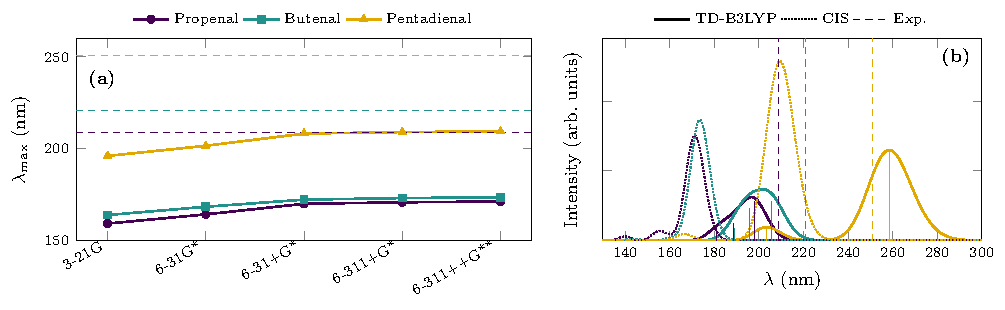
\includegraphics[scale=1]{figure_uv.pdf}
  \caption{(a) CIS wavelength of the $\pi\rightarrow\pi^*$ band against the
    basis set. (b) Spectra simulated with Gaussian functions
    ($\sigma = 0.25$~eV; illustrative band shapes, quantitative values in
    \cref{tab:lambda}) from TD-B3LYP (solid; vertical bars, individual
    transitions of height $f$) and CIS (dotted), both with 6-311++G**.
    Dashed lines: experimental maxima. Same colours in both panels.}
  \label{fig:uv}
\end{figure}


\textbf{TD-B3LYP: correlation removes most of the error.} TD-B3LYP reduces
the error to 7--15~nm (0.1--0.4~eV). Contrary to the hypothesis, however,
it does not systematically overshoot $\lambda_\mathrm{max}$: it falls short
for propenal and butenal and only overshoots for pentadienal. In other
words, its error changes with the length of the $\pi$ system: TD-B3LYP
predicts a red shift of 61~nm from propenal to pentadienal, against 42~nm
experimentally. This overestimation of the effect of conjugation is
consistent with the tendency of approximate functionals such as B3LYP to
over-delocalise the electron density in extended $\pi$
systems~\cite{Dreuw2005}.

In TD-B3LYP, the bright state is the second excited
state, as expected~\cite{guion56}, but its intensity is partly shared with
higher states ($f = 0.28$ for propenal and butenal, against 0.65 for
pentadienal): in butenal, the third state ($f = 0.23$) shifts the maximum
of the simulated band from 206 to 202~nm (\cref{fig:uv}b). The simulated
spectra also reproduce the stronger absorption of the longer chromophore
(hyperchromic effect).


\textbf{ZINDO: right for empirical reasons.} ZINDO gives the smallest
errors for propenal and butenal (2--3~nm), but this is not a sign of a
better physical description: it is a semiempirical method whose parameters
were fitted to reproduce experimental spectra~\cite{Ridley1973}. Even so,
like TD-B3LYP, it overshoots the red shift of pentadienal.

Two sources of error are common to all the methods. First, the HF/3-21G
geometry: Hartree--Fock overestimates the alternation between single and
double bonds, which reduces the delocalisation and raises the excitation
energy. Second, the calculated values are vertical excitations of an
isolated molecule, whereas the experimental maxima are band maxima,
probably measured in solution.

\section{Conclusion} %What can i conclude?

\begin{enumerate}
  \item CIS underestimates $\lambda_\mathrm{max}$ of the three aldehydes by
    38--48~nm (excitation energies 1.0--1.5~eV too high). Increasing the
    basis set does not fix it: the wavelengths converge from 6-31+G*
    onwards, but to values that remain far from experiment. The error comes
    from the lack of electron correlation, not from the basis set.
  \item Including correlation through TD-B3LYP reduces the error to
    7--15~nm (0.1--0.4~eV). Its error, however, depends on the length of
    the $\pi$ system: it falls short for propenal and butenal and
    overshoots for pentadienal, overestimating the effect of conjugation.
  \item ZINDO gives the closest values for the two shorter aldehydes, as
    expected from a method parametrised against experimental spectra. All
    the methods reproduce the red shift caused by the conjugation.
\end{enumerate}
\bibliographystyle{unsrt}
\bibliography{bibliografia}

\end{document}
